\documentclass[../main.tex]{subfiles}

\begin{document}
Until this point, the map resolution term has been used repeatedly. However, the term has not been formally defined. The aim of this section is to provide some insights about map quality and resolution measurements.

\subsection{Angular assignment error}
Provided that the ground truth angular assignment of the experimental particles is known, the estimated angular assignment of can be compared against it to calculate the average deviation of the estimation. However, the ground truth angular assignment is not known, as after all, that is the purpose of angular assignment. Nevertheless, a secondary angular assignment can be provided by some other method. Therefore, this measurement is interesting for comparing and consensuating various algorithms. Additionally, this metric can be useful when assessing an algorithm with artificially generated experimental images (Phantoms).

In the case of comparing the results of two refinement algorithms, it is probable that the reconstructed volumes may not have the same orientation. This will induce a constant error on this metric. To avoid this error, the reconstructed volumes should be aligned to one another before comparing angles.

\subsection{Fourier Shell Correlation}
When there is no other estimation about the angular assignment, the prior method can not be used. Moreover, the angular error does not explicitly provide any information about the quality of the reconstructed volume. The \gls{fsc} tries to solve these issues by measuring the resolution of the reconstructed volume\cite{sorzano2017a}.

The \gls{fsc} is calculated by splitting the angular assigned particle set into two equally sized random subsets and generating a volume from each of the subsets. Then spherical surfaces (shells) are extracted from the Fourier transforms of the volumes, each one of them representing a certain frequency band. Comparing all shell pairs with the correlation metric, a correlation value can be assigned to each frequency band. This correlation in function of the frequency is known as the \gls{fsc}, which is expressed in the equation \eqref{eq:3:fsc} \cite{dubach2020}\cite{sorzano2017a}.

\begin{equation}\label{eq:3:fsc}
    FSC(\omega) =   \frac{
                        \sum_{\omega_i \in \omega} F_1(\omega_i) \cdot F_2(\omega_i)^*
                    }{
                        \sqrt{\sum_{\omega_i \in \omega} |F_1(\omega_i)|^2 \cdot \sum_{\omega_i \in \omega} |F_2(\omega_i)|^2}
                    }
\end{equation}

Typically, the \gls{fsc} tends to have a low-pass behaviour, as the \gls{snr} is worse at high frequency. This empirical fact is shown in the Figure \ref{fig:3:fsc}.  In fact, There is a direct relation between the \gls{fsc} and the \gls{ssnr}. The expression \eqref{eq:3:ssnr} suggests that the \gls{fsc} is proportional to the signal power, whilst the complement of the \gls{fsc} refers to the noise power.

\begin{equation}\label{eq:3:ssnr}
    SSNR(\omega) = \frac{FSC(\omega)}{1 - FSC(\omega)} \Leftrightarrow FSC(\omega) = \frac{SSNR(\omega)}{1 + SSNR(\omega)}
\end{equation}

\begin{figure}[htbp]
    \centering
    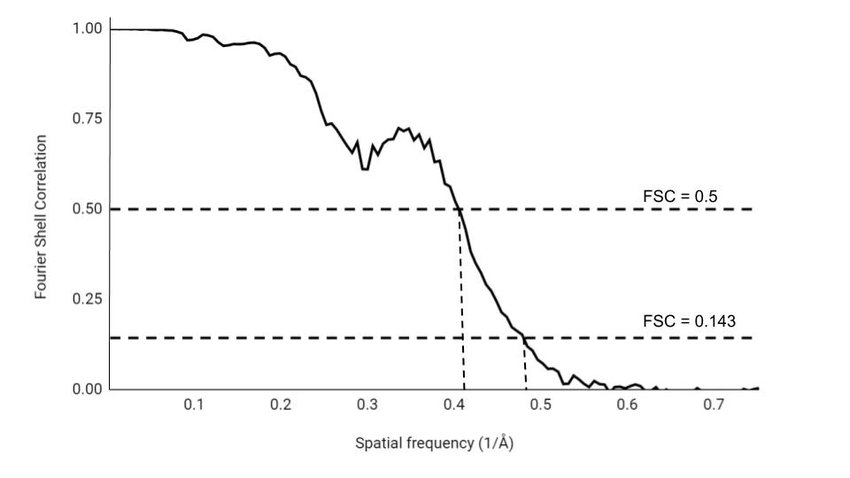
\includegraphics[width=\textwidth]{SPA/fsc}\\
    Image obtained from: \cite{dubach2020}
    \caption{Example of a FSC function}
    \label{fig:3:fsc}
\end{figure}

Due to this empirical low-pass tendency, it is useful to establish a threshold. In this way, the resolution of a map can be determined as the first value where this \gls{fsc} threshold is crossed. This provides a numerical value that unequivocally defines the quality of the map. The \gls{fsc} threshold value election is source for a long lived discussion in academia. Some experts argue that this threshold should be $0.5$, in reference to the cutoff frequency in the context of signal processing. Some other experts prefer to use $0.143$. This value reflects better the resolution of the map that would be obtained when considering the whole particle set (instead of halves)\cite{chen2013}. As a consequence of this debate, the threshold value used for determining the resolution of the map needs to be provided along the actual measurement.

\end{document}
